La Tabla \ref{tab:recorrido_auto} muestra la distancia que un automóvil recorre en el tiempo indicado.

\begin{multicols}{2}
    \begin{table}[H]
        \centering
        \caption{Datos sobre el recorrido de un automóvil}
        \label{tab:recorrido_auto}
        \begin{tabular}{|>{\columncolor{colorrds!80}\color{white}\bfseries}c|c|c|c|c|}
            \toprule
            Distancia (km) & 20            & 60             & 80 & 100            \\\cline{2-5}\midrule
            Tiempo (h)     & $\frac{1}{2}$ & 1$\frac{1}{2}$ & 2  & 2$\frac{1}{2}$ \\\cline{2-5}
            \bottomrule
        \end{tabular}
    \end{table}
    \begin{parts}
        \part Grafica en el plano cartesiano de la Figura \ref{fig:recorrido_auto} los puntos que indican
        los datos de la Tabla \ref{tab:recorrido_auto} y únelos con una línea.

        \vspace{-0.8cm}
        \begin{figure}[H]
            \centering
            \ifprintanswers
                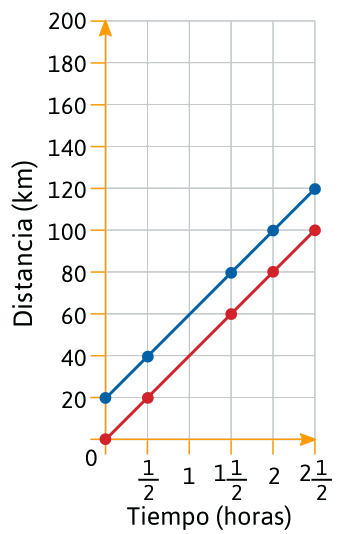
\includegraphics[width=0.46\linewidth]{../images/20230320220450}
            \else
                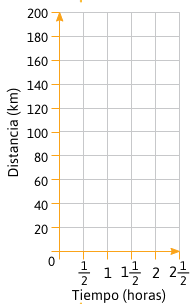
\includegraphics[width=0.46\linewidth]{../images/recorrido_auto_blank}
            \fi
            \caption{Gráfica del recorrido de un automóvil.}
            \label{fig:recorrido_auto}
        \end{figure}

        \part ¿La relación entre las variables corresponde a una relación de variación proporcional? ¿Por qué?

        \begin{solutionbox}{1.6cm}
            Sí es proporcional, ya que la razón de distancia recorrida entre tiempo es
            constante.
        \end{solutionbox}

        \columnbreak

        \part Si el automóvil pasa por el kilómetro cero y se mueve siempre con la misma velocidad, ¿qué distancia recorrerá en 4 horas?

        \begin{solutionbox}{1.2cm}
            160 km.
        \end{solutionbox}

        \part Dibuja en {\color{colorrds}color azul} en el plano cartesiano de la Figura \ref{fig:recorrido_auto} la gráfica que corresponda
        al movimiento de otro automóvil que cada hora recorre 20 km más que el
        primero y que inicia el recorrido al mismo tiempo.

        \begin{subparts}
            \subpart ¿La relación entre la distancia que recorre el segundo automóvil y el tiempo es de variación proporcional? ¿Por qué?

            \begin{solutionbox}{1.6cm}
                Si, ya que la variación entre la diastancia y el tiempo es constante.
            \end{solutionbox}

            \subpart ¿Los dos automóviles coinciden en algún momento? Si es así, ¿en qué momento sucede?

            \begin{solutionbox}{1.6cm}
                No, los automóviles no coinciden en ningún momento.
            \end{solutionbox}

            \subpart Si sólo conocieras las gráficas de ambos automóviles, ¿podrías determinar cuál es el más rápido? ¿Por qué?

            \begin{solutionbox}{1.6cm}
                Sí, por la inclinación de la recta.
            \end{solutionbox}
        \end{subparts}
        % Redacta una manera de obtener, a partir de la gráfica de la Figura \ref{fig:recorrido_auto}, la distancia que el
        % automóvil recorre en un tiempo dado.
    \end{parts}
\end{multicols}
% \end{minipage}
